\documentclass[a4paper]{article}

\usepackage[T1]{fontenc}
\usepackage[swedish]{babel}
\usepackage[utf8]{inputenc}
\usepackage{amsmath}
\usepackage{minted}
\usepackage{graphicx}
\title{Labb2 - Logik1351}

\author{Oliver Eriksson}

\date{\today}
\setcounter{section}{0}
\setcounter{tocdepth}{4}
\begin{document}
\maketitle
\newpage
\tableofcontents
\newpage

\section{Introduktion}
\label{sec:introduction}

Syftet med labben var att skriva ett program i Prolog som, givet en satslogisk konsekvens och ett bevis i naturlig deduktion, kunde avgöra om ett bevis var komplett och korrekt. Programmet skulle således returnera sant om beviset, utifrån de givna premisserna, naturligt och regelrätt gick att följa för att komma fram till slutsatsen. I alla andra fall skulle programmet returnera falskt.

Det rapporten kommer förklara är tillvägagångssättet för att skapa detta beskrivda program, samt diskutera huruvida programmet som tas fram är korrekt eller inte. Slutligen kommer jag även presentera två egna exempel på indata där resultatet är sant respektive falskt.

\section{Utförande}
För att lösa problemet användes till stor del uppgiftsbladet "labb2.pdf" där det huvudsakliga tipset jag utgick ifrån var "Börja med att lösa enkla exempel [..] När detta fungerar lägger du lämpligtvis till funktionalitet för övriga regler och slutligen hantering av boxar."

Inledningsvis implementerades därför \mintinline{prolog}{verify/1} enligt instruktionsbladet, så att programmet kan läsa in en fil och kalla funktionen \mintinline{prolog}{valid_proof/3} utifrån premisserna, slutsatsen och beviset själv. Denna funktion returnerar sant om och endast om filen går att läsa in samt om beviset är korrekt.

Därefter byggdes \mintinline{prolog}{valid_proof/3}, som först kollar om beviset inte är tomt. Ett tomt bevis säger ingenting, och därför får bevislistan inte vara tom. Därefter kollar \mintinline{prolog}{valid_proof/3} om \mintinline{prolog}{last(Proof, [_, Goal, _])}, vilket tittar om påståendet på sista raden i beviset är detsamma som vårt mål. Stämmer det börjar vi iterera igenom beviset med \mintinline{prolog}{iterate_proof/4}. Om \mintinline{prolog}{iterate_proof/4} i sin tur returnerar sant, betyder det att vårt bevis är komplett och \mintinline{prolog}{valid_proof/3} är sant.

\subsection{iterate\_proof/4}
\label{subsec:iterateproof}
\mintinline{prolog}{iterate_proof/4} är alltså predikatet som rekursivt itererar igenom vårt Proof. De fyra parametrarna består av problemets premisser, målet, en sublista till beviset över allt vi har kvar att iterera igenom samt sist hela beviset. Det \mintinline{prolog}{iterate_proof/4} därefter i huvudsak gör är att kolla vad som ligger längst upp i vårt bevis sublista. Vi kollar alltså på nästa instruktion och tittar vilket radnummer, vilket påstående samt vilken regel som används för att bevisa påståendet. Ett generellt exempel på hur \mintinline{prolog}{iterate_proof/4} används är: 
\begin{minted}{prolog}
iterate_proof(Prems, Goal, [[Row, Prop, Rule]|Rest], Proof) :-
	/*	Logik för hur Rule ska 
	* 	valideras givet Prop och Row 
	*/
	iterate_proof(Prems, Goal, Rest, Proof).
\end{minted}
På detta sätt kontrollerar vi varenda regel linjärt men rekursivt ner i vårt bevis givet att det inte finns några boxar. Om vi lyckas följa \mintinline{prolog}{iterate_proof/4} tills listan Rest är tom, alltså när prolog kan bevisa \mintinline{prolog}{iterate_proof(_, _, [], Proof)}, så kan vi konstatera att beviset håller för alla regler och därmed är fullständigt och regelrätt.

Implementationen av specifika regler sker därefter genom unifiering av en konstant. Till exempel vet vi att värdet för Rule är premise om prolog lyckas unifiera \mintinline{prolog}{iterate_proof(Prems, Goal, [[Row, Prop, Rule]|Rest], Proof)} med \mintinline{prolog}{iterate_proof(Prems, Goal, [[Row, Prop, impel(X,Y)]|Rest], Proof) :- ...} där X och Y är variabler som unifieras med värden till atomen impel. Denna regel skulle representera implikations-elimination, i vanlig predikatlogik. De regler som implementerades på detta sätt var samtliga som står listade under A.2 Regelappliceringar i labb2.pdf-bladet. 

En viktig sak att poängtera är att \mintinline{prolog}{iterate_proof/4} automatiskt misslyckas om den sista raden i beviset inte innehåller slutsatsen, samt om sista raden inte är ett antagande.

\begin{minted}{prolog}
iterate_proof(_, Goal, [[Row, Prop, Rule]|[]], Proof) :-
        last(Proof, [Row, Prop, _]),
        \+(Rule = assumption),
        \+(Prop = Goal), !,
        fail.
\end{minted} 
Anledningen att det inte får vara ett antagande på sista raden är för att det är okej att öppna en låda med endast ett antagande, där alltså både första och sista raden innehåller ett antagande. Vi vill alltså inte automatiskt falsifiera bevis där det finns outnyttjade självstående antaganden. Samtliga reglers fullständiga implementationer går att läsa i predikattabellen senare i rapporten.

\subsection{search\_line/4} \label{subsec:searchline}
För att därefter kunna kontrollera om en regel använts korrekt implementerades först och främst predikatet \mintinline{prolog}{search_line/4} vars främsta funktion är att finna satsen Prop på raden \mintinline{prolog}{Prop_row} givet regelns rad \mintinline{prolog}{Call_row}. 

\begin{minted}{prolog}
search_line(Call_row, Prop_row, Prop, [[Prop_row, Prop, _]|Rest], Proof) :- 
	valid_boxing(Prop_row, Call_row, Proof).
search_line(Call_row, Prop_row, Prop, [Box|_], Proof) :-
	search_line(Call_row, Prop_row, Prop, Box, Proof).
search_line(Call_row, Prop_row, Prop, [_|Rest], Proof) :-
	search_line(Call_row, Prop_row, Prop, Rest, Proof).
\end{minted}

När prolog lyckas unifiera parametrarna i \mintinline{prolog}{search_line/4} med 
\begin{minted}{prolog}
search_line(Call_row, Prop_row, Prop, [[Prop_row, Prop, _]|Rest], Proof),
\end{minted}
alltså när vi har hittat den rad i beviset med radnummer \mintinline{prolog}{Prop_row} och som samtidigt har satsen Prop, då säger vi att \mintinline{prolog}{search_line/4} är sann om 
\begin{minted}{prolog}
valid_boxing(Prop_row, Call_row, Proof)
\end{minted}
är sann. Det vill säga, \mintinline{prolog}{search_line/4} är sann om och endast om vi kan hitta en rad i beviset som innehåller radnumret \mintinline{prolog}{Prop_row}, om vi på samma rad också unifiera \mintinline{prolog}{Prop} samt om det är möjligt att gå från \mintinline{prolog}{Prop_row} till \mintinline{prolog}{Call_row} med accepterade förflyttningar genom olika boxar, vilket testas med \mintinline{prolog}{valid_boxing/3}.

\mintinline{prolog}{valid_boxing(R1,R2,Proof)} är väldigt rak på sak, och fungerar så att vi väljer ut den av R1 eller R2 som är minst, därefter skickar vi in den minsta av dessa (Alltså den raden som kommer först i beviset) tillsammans med Proof till \mintinline{prolog}{findRowIn/3}, som letar reda på den rad i beviset som innehåller detta minsta radnummer, och returnerar resten av beviset från den raden. Givet resten av beviset från R1 (om R1 är mindre än R2), tittar vi då om det är möjligt att gå till R2.

\begin{minted}{prolog}
valid_boxing(R1, R2, Proof) :-
	R1 < R2,
	findRowIn(R1, Proof, Rest),
	findRowIn(R2, Rest, _);
	R2 < R1,
	findRowIn(R2, Proof, Rest),
	findRowIn(R1, Rest, _).

findRowIn(Row, [[Row, P, R]|Rest], [[Row, P, R]|Rest]).
findRowIn(Row, [[H|T]|Proof], Rest) :-
	findRowIn(Row, [H|T], Rest).
findRowIn(Row, [_|Proof], Rest) :-
	findRowIn(Row, Proof, Rest).
\end{minted}
På grund av implementationen av findRowIn, som endast kan välja att hoppa in i en box, eller skippa en box, kommer vi endast lyckas hitta R2 givet R1 om R2 är på en högre nestad nivå eller samma nivå som R1. Vi kommer således aldrig kunna hämta R1 och R2 från två olika boxar, och kommer heller aldrig kunna hämta R1 från R2 om R1 ligger efter och utanför boxen som R2 befinner sig i.

Fördelen med att \mintinline{prolog}{findRowIn/3} returnerar restlistan inklusive raden med det radnummer vi söker är att detta senare kan användas för att bekräfta en korrekt implementerad box.

\subsection{search\_box/6}
När väl \mintinline{prolog}{search_line/4} var implementerad byggdes \mintinline{prolog}{search_box/6}. Detta predikat kollar första och sista raderna i en box som introducerats tidigare. Kravet på "tidigare" är här att boxen som kontrolleras måste finnas i samma box som regeln vilken refererar till denna kontrollerade box.
\begin{minted}{prolog}
search_box(Call_row, BStart_row, BStart_prop, BEnd_row, BEnd_prop, Proof) :-
	call_row_after_box( BStart_row, Call_row, Proof ),
	findRowIn(BStart_row, Proof, Rest),
	last(Rest, [BEnd_row, BEnd_prop, _]),
	first(Rest, [BStart_row, BStart_prop, _]).
\end{minted}
Med andra ord måste \mintinline{prolog}{Call_row} ligga efter den box som \mintinline{prolog}{BStart_row} är första radnummer och \mintinline{prolog}{BEnd_row} är sista radnummer till. Ett exempel följer:
\begin{minted}{prolog}
[
	[1, Prop,	Rule],
	[
		[BStart_row, BStart_prop, Rule],
		.
		.
		.
		[BEnd_row, BEnd_prop, Rule],
	]
	[N, Prop, Rule],
	[Call_row, Prop, Rule(BStart_row, BEnd_row)]
].
\end{minted}
Denna struktur är således den enda struktur som tillåts och som således gör 
\begin{minted}{prolog}
search_box(Call_row, BStart_row, BStart_prop, BEnd_row, BEnd_prop, Proof) :-
        call_row_after_box( BStart_row, Call_row, Proof ),
        findRowIn(BStart_row, Proof, Rest),
        last(Rest, [BEnd_row, BEnd_prop, _]),
        first(Rest, [BStart_row, BStart_prop, _]).
\end{minted}
sann. Hur predikatet fungerar är att \mintinline{prolog}{call_row_after_box/3} kontrollerar så att \mintinline{prolog}{Call_row} endast går att hitta samma box som rad 1, N och \mintinline{prolog}{Call_row} i exemplet ovan. Därefter letar findRowIn, givet \mintinline{prolog}{BStart_row} och Proof, reda på resten av beviset från och med \mintinline{prolog}{BStart_row}, som beskrivet i \ref{subsec:searchline}. Givet resten av beviset, vilken endast kommer innehålla rader från den önskade boxen, hämtar vi den första och sista raden och garanterar oss om att dessa innehåller de formler som är givna i \mintinline{prolog}{BStart_prop} och \mintinline{prolog}{BEnd_prop}.

\subsection{Box-branch}
Förutom hur boxarna är implementerade och hur de bevisas korrekta, var det även nödvändigt att definiera hur vi känner igen en box när vi itererar genom beviset med \mintinline{prolog}{iterate_proof/4}. Sättet jag löste problemet på var att definiera

\begin{minted}{prolog}
iterate_proof(Prems, Goal, [[[Row, Prop, assumption]|NextInBox] | Rest], Proof) :-
        iterate_proof(Prems, Goal, NextInBox, Proof),
        iterate_proof(Prems, Goal, Rest, Proof).
\end{minted}
som säger att om vi stöter på en rad där första elementet är en lista vars första element i sin tur har regeln ``assumption``, då måste \mintinline{prolog}{iterate_proof/4} vara sant både om vi itererar igenom den inre listan såväl som resten av beviset utanför denna nestade lista. 

Med andra ord stöter vi på en box om och endast om första regeln i en nestad lista är ett antagande. I ett sådant fall måste vi kunna följa såväl sublistan som resten av beviset och komma fram till att båda bevisen enskilt är sanna. Detta är rekursivt möjligt eftersom ett bevis/subbevis är sant om och endast om vi i slutet av respektive bevis kan unifiera \mintinline{prolog}{iterate_proof(_, _, [], Proof)}, som förklarat i \ref{subsec:iterateproof}.

\subsection{Regler}
För att implementera alla regler i Figur \ref{fig:ruletable} användes alla ovan nämnda predikat i olika kombinationer. Hur reglerna är implementerade står förklarade i \ref{subsec:iterateproof} genom predikatet \mintinline{prolog}{iterate_proof/4}. Själva konkreta implementationen samt när alla predikat är sanna finns listad i Appendix A.

\begin{figure}[!h]
  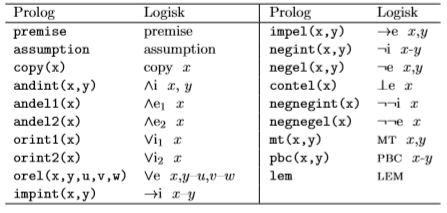
\includegraphics[]{ruletable.png}
  \caption{En kopia av alla regler från labb2.pdf}
  \label{fig:ruletable}
\end{figure}

\section{Diskussion}
Programmet som skrevs kan slutligen passera alla de tester som var en del i uppgiftsunderlaget, alltså valid01-valid21 samt invalid01-invalid28. Jag bedömer att det bekräftar att programmet håller för de allra flesta bevis. 

En viktig sak att tillägga är dock att alla regler inte är kommutativt definierade. Ett exempel som nu är åtgärdat, men som från början
inte fungerade korrekt även om alla testfall lyckades, var att LEM för or(P, neg(P)) returnerade sant, men LEM för or(neg(P), P) var falskt. Detsamma gäller fortfarande för t.ex orel, vilket är beskrivet som kommentar i programkoden för predikatet i Appendix A. Problemet är där att
det spelar roll för orel(X,Y,Z,U,V) om box Y-Z förekommer före eller efter U-V i programmet givet de antaganden och slutsatser som är kopplade till respektive box.

I övrigt fungerar det mesta som det ska.
\newpage
\section{Appendix A. Programkod}
Appendix A innehåller all programkod inklusive kommentarer som beskriver när varje predikat är sant/falskt.

\begin{minted}{prolog}
/**
        Enter url to input-file where:
        Prems - All premises on the form [A, B, ...,E].
        Goal - The goal formed as a Propositional logic expression
        Proof - The proof on the form [[Row, Proposition, Rule], ..., [Row, Goal, Rule]]
*/
verify(InputFileName) :- see(InputFileName),
        read(Prems), read(Goal), read(Proof),
        seen,
        valid_proof(Prems, Goal, Proof).

/**
        A proof is valid if the last element of the proof contains the Goal,
        the proof is not empty and we can iterate, using rules of Natural Deduction,
        through the proof reaching the end of it.
*/
valid_proof(Prems, Goal, Proof) :-
        \+is_empty(Proof),
        last(Proof, [_, Goal, _]),
        iterate_proof(Prems, Goal, Proof, Proof).

/**
        If we hit the last row of the proof and Prop != Goal, then the proof failed.
        Also if we hit the last row and the Rule is an assumption, the proof fails.
*/
iterate_proof(_, Goal, [[Row, Prop, Rule]|[]], Proof) :-
        last(Proof, [Row, Prop, _]),
        \+(Rule = assumption),
        \+(Prop = Goal), !,
        fail.

/**
        This signifies that a proof inside a box has reached its end. 
        (could also be box of whole proof)

        In this case, iterate_proof is VALID, and we will either continue at #split,
        or consider that the proof holds.
*/
iterate_proof(_, _, [], Proof).

/**     PREMISE

        If the rule is "premise", then check whether the current
        proposition is in the premis-list, if true, continue iterating.
        
        True if: Prop is a member of the list of premises, 
        and if the rest of the proof is true
*/
iterate_proof(Prems, Goal, [[Row, Prop, premise]|Proof_rest], Proof) :-
        member(Prop, Prems), !,
        iterate_proof(Prems, Goal, Proof_rest, Proof).

/**     And-Introduction

	True if: We can find Prop A at row X and B at row Y while
	X and Y are smaller than the row of the rule.
		
	Also, the rest of the proof has to be true.
*/
iterate_proof(Prems, Goal, [[Row, and(A,B), andint(X,Y)]|Rest], Proof) :-
        search_line(Row, X, A, Proof, Proof),
        search_line(Row, Y, B, Proof, Proof),
        X < Row, Y < Row,
        iterate_proof(Prems, Goal, Rest, Proof);
        search_line(Row, X, B, Proof, Proof),
        search_line(Row, Y, A, Proof, Proof),
        X < Row, Y < Row,
        iterate_proof(Prems, Goal, Rest, Proof).

/**     And-Elimination-1

	True if: We can find and(Prop, _) on row X, where 
	X is smaller than the row of the rule
		
	Also, the rest of the proof has to be true.
*/
iterate_proof(Prems, Goal, [[Row, Prop, andel1(X)]|Rest], Proof) :-
        search_line(Row, X, and(Prop, _), Proof, Proof),
        X < Row,
        iterate_proof(Prems, Goal, Rest, Proof).

/**     And-Elimination-2

	See And-Elimination-1, but with and(_, Prop) as the Prop.

*/
iterate_proof(Prems, Goal, [[Row, Prop, andel2(X)]|Rest], Proof) :-
        search_line(Row, X, and(_, Prop), Proof, Proof),
        X < Row,
        iterate_proof(Prems, Goal, Rest, Proof).

/**     Or-Introduction-1

	True if: we can find proposition A on row X,
	where X is smaller than Row
		
	Also, the rest of the proof has to be true.
*/
iterate_proof(Prems, Goal, [[Row, or(A,_), orint1(X)]|Rest], Proof) :-
        search_line(Row, X, A, Proof, Proof),
        X < Row,
        iterate_proof(Prems, Goal, Rest, Proof).

/**     Or-Introduction-2

	True if: we can find proposition B on row X,
	where X is smaller than Row
		
	Also, the rest of the proof has to be true.
*/
iterate_proof(Prems, Goal, [[Row, or(_,B), orint2(X)]|Rest], Proof) :-
        search_line(Row, X, B, Proof, Proof),
        X < Row,
        iterate_proof(Prems, Goal, Rest, Proof).

/**     Implication-Elimination

	True if: Rule is impel(x,y) then search and check whether row Y
	contains the proposition imp(T,Prop) where Prop is our current prop.
	Also check whether row X contains the element T in T -> Prop.
        
	The rest of the proof also has to be true.
*/
iterate_proof(Prems, Goal, [[Row, Prop, impel(X,Y)]|Proof_rest], Proof) :-
        search_line(Row, Y, imp(T,Prop), Proof, Proof),
        search_line(Row, X, T, Proof, Proof),
        X < Row, Y < Row,
        iterate_proof(Prems, Goal, Proof_rest, Proof).

/**     Implication-Introduction
	
	True if: We can find a box starting on row X ending on row Y where
	the proposition on X is BoxStart and the proposition on Y is
	BoxEnd.
        
	The rest of the proof also has to be true.
*/
iterate_proof(Prems, Goal, [[Row, imp(BoxStart,BoxEnd), impint(X,Y)]|Rest], Proof) :-
        search_box(Row, X, BoxStart, Y, BoxEnd, Proof),
        iterate_proof(Prems, Goal, Rest, Proof).
/**	Or-Elimination
	
	True if: We can find a proposition on the form "or(A,B)" on row X, where
	X is smaller than the row of the rule. We also need to make sure that
	we can find a box starting on row U with proposition A, ending on row
	V with proposition Prop. Moreover, there has to be another box starting on
	row P with proposition B, ending on row Q which also has to contain proposition
	Prop. If we can find those to boxes and the line including or(A,B), we
	can be sure that the rule holds.
	
	The rest of the proof also has to be true.
	
	This function might need to be changed to also try reversed order of A and B.
	It might be the case that the A is the assumption of the box P-Q and not U-V.
	This is not attempted now, and the proposition will therefore fail in that case.
	
	The proposition is not commutative around or(A,B) in this implementation.
*/
iterate_proof(Prems, Goal, [[Row,Prop, orel(X,U,V,P,Q)]|Rest], Proof) :-
        search_line(Row, X, or(A,B), Proof, Proof),
        X < Row,
        search_box(Row, U, A, V, Prop, Proof),
        search_box(Row, P, B, Q, Prop, Proof),
        iterate_proof(Prems, Goal, Rest, Proof).

/**     Negation-Introduction

	True if: We can find Prop on row X where neg(Prop) is found on row
	Row.
	
	Also, the rest of the proof has to hold.
*/
iterate_proof(Prems, Goal, [[Row, neg(Prop), negint(X,Y)]|Rest], Proof) :-
        search_box(Row, X, Prop, Y, cont, Proof),
        iterate_proof(Prems, Goal, Rest, Proof).

/**     Negation-Elimination

	True if: We can find both proposition Prop on row X and neg(Prop)
	on row Y where both X and Y are less than Row.
	
	This predicate is implemented to be commutative as my neg-predicate
	is naive.
*/
iterate_proof(Prems, Goal, [[Row, cont, negel(X,Y)]|Rest], Proof) :-
        search_line(Row, X, Prop, Proof, Proof),
        search_line(Row, Y, neg(Prop), Proof, Proof),
        X < Row, Y < Row,
        iterate_proof(Prems, Goal, Rest, Proof);
        search_line(Row, X, neg(Prop), Proof, Proof),
        search_line(Row, Y, Prop, Proof, Proof),
        X < Row, Y < Row,
        iterate_proof(Prems, Goal, Rest, Proof).

/**     Contradiction-Elimination

	True if: We can find cont on row X, then Prop can be anything.
	X has to be smaller than Row, and the rest of the proof has to be true.
*/
iterate_proof(Prems, Goal, [[Row, Prop, contel(X)]|Rest], Proof) :-
        search_line(Row, X, cont, Proof, Proof),
        X < Row,
        iterate_proof(Prems, Goal, Rest, Proof).

/**     Double-Negation-Introduction

	True if: we on row X can find A, then we are allowed 
	to introduce neg(neg(A))
*/
iterate_proof(Prems, Goal, [[Row, neg(neg(A)), negnegint(X)]|Rest], Proof) :-
        search_line(Row, X, A, Proof, Proof),
        X < Row,
        iterate_proof(Prems, Goal, Rest, Proof).

/**     Double-Negation-Elimination

	True if: we on row X can find neg(neg(Prop), then we are allowed
	to eliminate neg(neg(Prop) and state Prop.
*/
iterate_proof(Prems, Goal, [[Row, Prop, negnegel(X)]|Rest], Proof) :-
        search_line(Row, X, neg(neg(Prop)), Proof, Proof),
        X < Row,
        iterate_proof(Prems, Goal, Rest, Proof).

/** Modus Tollens
        (P -> Q), !Q |- !P
        
	True if: We on line X can find imp(P,Q) 
	and if we can find neg(Q) on line Y.
	X and Y are smaller than row. 
     
	Also, the rest of the proof has to hold.    
*/
iterate_proof(Prems, Goal, [[Row, neg(P), mt(X,Y)]|Rest], Proof) :-
        search_line(Row, X, imp(P,Q), Proof, Proof),
        search_line(Row, Y, neg(Q), Proof, Proof),
        X < Row, Y < Row,
        iterate_proof(Prems, Goal, Rest, Proof).

/**     LEM
        |- (A OR !A)
        
        True if: The rule is LEM and the prop is either or(P, neg(P),
        or or(neg(P), P)
*/
iterate_proof(Prems, Goal, [[Row, or(P, neg(P)), lem]|Rest], Proof) :-
        iterate_proof(Prems, Goal, Rest, Proof).
iterate_proof(Prems, Goal, [[Row, or(neg(P), P), lem]|Rest], Proof) :-
        iterate_proof(Prems, Goal, Rest, Proof).

/**
        #Split
        In case we encounter a box-opening, we need to iterate into 
        both the box and the rest of the proof.
        
        True if: There is a nested list in the head of the list where the Rule
        is "assumption", then we want to iterate into both the Box and
        into the rest of the proof. Both routes have to be true for
        this predicate to be valid.
*/
iterate_proof(Prems, Goal, [[[Row, Prop, assumption]|NextInBox] | Rest], Proof) :-
        iterate_proof(Prems, Goal, NextInBox, Proof),
        iterate_proof(Prems, Goal, Rest, Proof).

/**     COPY
        Lets us copy something already proved into a later stage of the proof
        
        True if: there is any prop at row X and that X is smaller than row.
        
        The rest of the proof also has to be true.
*/
iterate_proof(Prems, Goal, [[Row, Prop, copy(X)]|Rest], Proof) :-
        search_line(Row, X, Prop, Proof, Proof),
        X < Row,
        iterate_proof(Prems, Goal, Rest, Proof).

/**     Proof-By-Contradiction
        Assuming not(Prop) and being able to show a Contradiction
        lets us conclude that Prop is true.
        
        True if: We can find a box starting on X containing neg(Prop) 
        where Prop is an arbitrary proposition. The box starting on row X
        also has to end on row Y containing cont, stating a contradiction
        was found.
        
        The rest of the proof also has to be true.
*/
iterate_proof(Prems, Goal, [[Row, Prop, pbc(X,Y)]|Rest], Proof) :-
        search_box(Row, X, neg(Prop), Y, cont, Proof),
        iterate_proof(Prems, Goal, Rest, Proof).

/**     search_box

        Lets us, given a rule on row "Call_row", check whether
        a box starting on BStart_row and ending on BEnd_row is
        valid, contains the Propositions we assume and accessible from Call_row.
        
        True if: See description under 2.3 search_box/6 in report
*/
search_box(Call_row, BStart_row, BStart_prop, BEnd_row, BEnd_prop, Proof) :-
        call_row_after_box( BStart_row, Call_row, Proof ),
        findRowIn(BStart_row, Proof, Rest),
        last(Rest, [BEnd_row, BEnd_prop, _]),
        first(Rest, [BStart_row, BStart_prop, _]).

/** A simple predicate telling if H is the first element of a List 
	
	True if: the second argument is unifiable with the head of the list 
	passed as first argument.
*/
first([H|T], H).

/**
        Lets us check whether a rownumber is in the same box as a specific box.
        i.e:
        [a
                [b,
                        [c,
                        d],
                e]
        f]
        The proposition tells us if for example the box c-d is 
        accessible from a row X. 
        
        True if: X = e and Boxstart = c or X = f and Boxstart = b, the proposition in this 
        case is true. Any other variable combination would return false.
*/
call_row_after_box(Boxstart, Callrow, [[[Boxstart, _, _]|Boxrest]|Rest]) :-
        member([Callrow,_,_], Rest).
call_row_after_box( Boxstart, Callrow, [H|Rest] ) :-
        call_row_after_box( Boxstart, Callrow, Rest).
call_row_after_box( Boxstart, Callrow, [H|Rest] ) :-
        call_row_after_box( Boxstart, Callrow, H ).

/**
        Looks for a specific "line"/proofrow in the Proof.
        If it is found, and it is found through valid_boxing,
        then search_line is true.
        
        True if: For further explanation, see 2.2 in report.
*/
search_line(Call_row, Prop_row, Prop, [[Prop_row, Prop, _]|Rest], Proof) :- 
		valid_boxing(Prop_row, Call_row, Proof).
search_line(Call_row, Prop_row, Prop, [Box|_], Proof) :-
        search_line(Call_row, Prop_row, Prop, Box, Proof).
search_line(Call_row, Prop_row, Prop, [_|Rest], Proof) :-
        search_line(Call_row, Prop_row, Prop, Rest, Proof).

/**
        A boxing is valid if we can find a row R2
        given the Rest of the proof following R1 iterating
        sequentially through Rest.
        
        True if: See 2.2 in report
*/
valid_boxing(R1, R2, Proof) :-
        R1 < R2,
        findRowIn(R1, Proof, Rest),
        findRowIn(R2, Rest, _);
        R2 < R1,
        findRowIn(R2, Proof, Rest),
        findRowIn(R1, Rest, _).

/**     Looks for a certain row of a proof and returns the rest of the proof given
        that found row.
        
        True if: see 2.2 in report
*/
findRowIn(Row, [[Row, P, R]|Rest], [[Row, P, R]|Rest]).
findRowIn(Row, [[H|T]|Proof], Rest) :-
        findRowIn(Row, [H|T], Rest).
findRowIn(Row, [_|Proof], Rest) :-
         findRowIn(Row, Proof, Rest).

/** Tells if a list is empty 
	
	True if: the argument is an empty list
	Fails if: The argument is any list containing more than one element
*/
is_empty([]).
is_empty([_,_]) :- fail.

/** Implements the Implication-proposition 
	
	Fails if: imp(fail, true)
	True if: any other combination of true/fail
*/
imp(P, true).
imp(fail, fail).

/** Implements logical-And 

	True if: Both P and Q are true, false otherwise
*/
and(P, Q) :- P, Q.

/** Implements logical-Or 
	
	True if: Either P or Q (or both) are true.
	Fails if: Neither are true
*/
or(P, true).
or(true, Q).

/** Implements negation 

	True if: We cannot prove X using prolog's negation as failure.
*/
neg(X) :- \+X.
\end{minted}
\newpage
\section{Appendix B. Exempelbevis}
Det första beviset är ett sant bevis som bygger på tautologin 
\begin{equation}
\vdash \phi \wedge (\psi \vee \delta) \rightarrow (\phi \wedge \psi) \vee \delta.
\end{equation}
Enligt programmets input-syntax implementerades följande bevis som exempel på ett korrekt bevis:
\begin{minted}{prolog}
/* Valid proof */
[].
imp( and(p,or(q,r)) , or(and(p,q),r) ).
[
	[
		[1,and(p,or(q,r)),assumption],
		[2,p,andel1(1)],
		[3,or(q,r),andel2(1)],
		[	
			[4,q,assumption],
			[5,and(p,q),andint(2,4)],
			[6,or(and(p,q),r),orint1(5)]
		],[
			[7,r,assumption],
			[8,or(and(p,q),r),orint2(7)]
		],
		[9,or(and(p,q),r),orel(3,4,6,7,8)]
	],
	[10,imp( and(p,or(q,r)) , or(and(p,q),r) ), impint(1,9)]	
].
\end{minted}
När beviset körs i programmet returnerar programmet true.

Ett exempel på ett felaktigt bevis skulle vara om vi påstod $\phi \vdash \psi$,
detta implementerades som ett motsägelsebevis genom:
\begin{minted}{prolog}
/* Invalid proof */
[p].
t.
[	
	[1, p, premise],
	[
		[2, neg(p), assumption],
		[3, p,	copy(1)],
		[4, cont, negel(2,3)]
	],
	[5, cont, copy(4)],
	[6, t, contel(5)]
].
\end{minted}
Detta bevis returnerar falskt eftersom mitt program inte tillåter att kopiera från en rad på en högre box-nivå raden där copy själv används, vilket är sunt. Annars skulle vi som enligt detta exempel kunna kopiera godtyckliga påståenden och bevisa sanna saker från t.ex godtyckliga antaganden.

Om prologs inbyggda "trace"-program körs i bakgrunden kan man se att programmet misslyckas när den försöker bevisa rad 5 och därmed returnerar false.
\end{document}